\section{UML}

Voici dans la \ref{fig:uml} le diagramme de classe décrivant les données nécessaires à la gestion de l'emploi du temps.
Comme on peut le constater, on regroupe l'ensemble des données nécessaires et déterminées à l'avance dans des Séances. A savoir : le(s) groupe(s) d'étudiants concerné(s), le professeur, la matière, ainsi que le type de cours. Ensuite ces séances vont être associées à des créneaux par notre solution. Les créneaux étant le regroupement d'un jour, une plage horaire et une salle.
Un peu noter des détails intéressants, sur Groupe, il y a la notion d'incompatibilité qui permet de définir lorsqu'il est possible pour deux groupes d'avoir cours sur une même plage horaire. Sur matière on à la notion de suite, lorsqu'une matière débute après la fin d'une autre (cf Mini-Projet d'IA qui suit le cours d'IA). Et enfin sur séance, on a la notion de suite aussi qui décrit une nombre de jours minimum et maximum avant le prochain cours de la même matière.

\begin{landscape}

        \begin{figure}[t]
            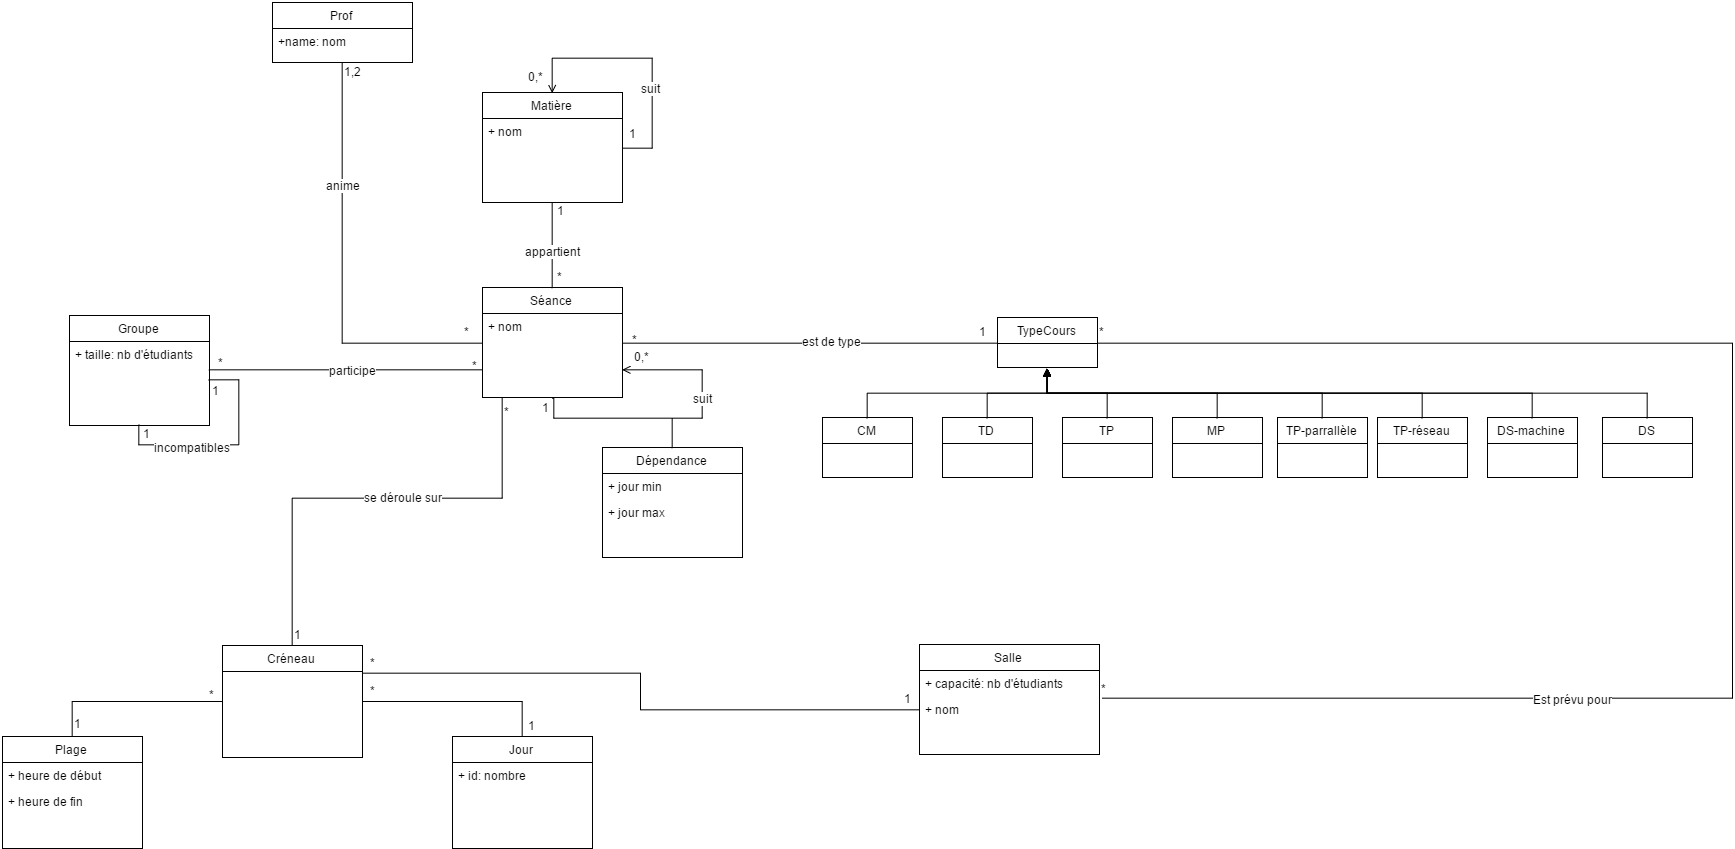
\includegraphics[keepaspectratio=true,width=26cm]{diagrammeClasse.png}
            \caption{\label{fig:uml} Modélisation UML}
        \end{figure}

\end{landscape}
